\documentclass{easychair}

%%%%%%%%%%%%%%%%%%%%%%%%%%%%%%%%%%%%%%%%%%%%%%%%%%%%%%%%%%%%%%%%%%%%%%%%
%% Packages
%%%%%%%%%%%%%%%%%%%%%%%%%%%%%%%%%%%%%%%%%%%%%%%%%%%%%%%%%%%%%%%%%%%%%%%%

\usepackage[utf8]{inputenc}         % text encoding
\usepackage{amsmath}
\usepackage{amssymb}
\usepackage{amsthm}
\usepackage{amsfonts}               % \mathbb, \mathcal
\usepackage[algoruled]{algorithm2e} % \begin{algorithm}
\usepackage{lmodern}                % good replace for computer modern
\usepackage{bm}                     % \boldsymbol
\usepackage{xcolor}
\usepackage{placeins}               % \FloatBarrier
%\usepackage{parskip}

% number only those equations that get ref'd somewhere
\usepackage{mathtools}
\mathtoolsset{
  showonlyrefs=true % or false in draft mode
}

%%%%%%%%%%%%%%%%%%%%%%%%%%%%%%%%%%%%%%%%%%%%%%%%%%%%%%%%%%%%%%%%%%%%%%%%
%% New Commands
%%%%%%%%%%%%%%%%%%%%%%%%%%%%%%%%%%%%%%%%%%%%%%%%%%%%%%%%%%%%%%%%%%%%%%%%

\newcommand\ZZ{\mathbb{Z}}  % integers
\newcommand\QQ{\mathbb{Q}}  % rationals
\newcommand\RR{\mathbb{R}}  % reals

\renewcommand\v[1]{\boldsymbol{#1}}
\newcommand\mat[1]{\mathbf{#1}}
\newcommand\m[1]{\mathbf{#1}}
\newcommand\proc[1]{\textsc{#1}}

\DeclarePairedDelimiterX{\norm}[1]{\lVert}{\rVert}{#1}
\DeclarePairedDelimiterX{\abs}[1]{\lvert}{\rvert}{#1}
\newcommand\norminf[1]{\norm{#1}_\infty}
\DeclareMathOperator{\vol}{vol}

\newcommand\La{\mathcal{L}}  % Lattice
\newcommand\Co{\mathcal{C}}  % Constraints
\newcommand\linf{L^\infty}   % \infty-norm/metric
\newcommand{\ltwo}{L^2}
\newcommand\tz{\tilde{\v{z}}}
\newcommand{\fn}[1]{\mathrm{#1}}

\newcommand{\floor}[1]{\lfloor #1 \rfloor}
\newcommand{\ceil} [1]{\lceil  #1 \rceil}


%%%%%%%%%%%%%%%%%%%%%%%%%%%%%%%%%%%%%%%%%%%%%%%%%%%%%%%%%%%%%%%%%%%%%%%%
%% New Theorems
%%%%%%%%%%%%%%%%%%%%%%%%%%%%%%%%%%%%%%%%%%%%%%%%%%%%%%%%%%%%%%%%%%%%%%%%

\theoremstyle{plain}

\newtheorem{thm}{Theorem}[section]
\newtheorem{lem}[thm]{Lemma}
\newtheorem{prop}[thm]{Proposition}


\setlength{\parindent}{0em}
\setlength{\parskip}{6pt}

%%%%%%%%%%%%%%%%%%%%%%%%%%%%%%%%%%%%%%%%%%%%%%%%%%%%%%%%%%%%%%%%%%%%%%%%
%% Content
%%%%%%%%%%%%%%%%%%%%%%%%%%%%%%%%%%%%%%%%%%%%%%%%%%%%%%%%%%%%%%%%%%%%%%%%

\begin{document}

\title{Bounded Integer Linear Constraint Solving \\
       via Lattice Search}
\titlerunning{Bounded Integer Linear Constraint Solving}
\author{Joe Hendrix \and Benjamin F Jones}
\institute{Galois Inc., Portland,OR \\
    \email{jhendrix@galois.com, bjones@galois.com}}
\authorrunning{J. Hendrix and B. Jones}

\maketitle

\begin{abstract}

\setlength{\parskip}{6pt}

\noindent{}We present a novel algorithm for solving integer linear constraint
problems of the form $\v{l} \le \mat{A} \v{x} \le \v{u}$. Our approach is based
on techniques used to solve the closest vector problem for lattices, but adapted
to use the $\linf{}$ distance metric. We have implemented this algorithm in a
constraint solver called BLT.

\noindent{}The BLT solver was motivated by efforts to apply SMT solvers to
signal processing algorithms.  In particular, we describe here the problem of
\emph{reversing JPEG}, that is, finding compressed data that decompress into an
image satisfying given constraints.  This problem can be expressed as a bounded
integer linear constraint problem, but was intractable to the SMT solvers we
tried.  In contrast, BLT is able to solve many of the examples in seconds,
including both SAT and UNSAT problems.

\end{abstract}

%% Introduction %%%%%%%%%%%%%%%%%%%%%%%%%%%%%%%%%%%%%%%%%%%%%%%%%%%%%%%%
\section{Introduction}
\label{sec:intro}

% What is essential to say?

In this paper, we present a decision procedure for solving systems of
integer linear constraints where each expression is subject
to both upper and lower bounds.  Such systems have the form:
%
\begin{equation}
    \label{eq:prob-inequalities}
    \begin{array}{ccccc}
        l_1    & \le & a_{11} x_1 + \cdots + a_{1n} x_n & \le & u_1 \\
        l_2    & \le & a_{21} x_1 + \cdots + a_{2n} x_n & \le & u_2 \\
        \vdots &     & \vdots                         &     & \vdots \\
        l_m    & \le & a_{m1} x_1 + \cdots + a_{mn} x_n & \le & u_m
    \end{array}
\end{equation}
%
where $l_i, u_i, a_{ij}$ are rational constants and the $x_i$ are unknown
integer variables.
%
As a more compact notation, we use $\v{l} \le \mat{A} \v{x} \le \v{u}$
to denote systems with this form.


% The problem is also
%known as \emph{integer linear programming} (ILP), though we are only concerned
%with the feasibility question here.

Our decision procedure is based on a variant of the Schnorr-Euchner
algorithm~\cite{Schnorr-Euchner} for computing the closest lattice
element to a target point, and is implemented in a tool which we call
\emph{BLT}.  The decision procedure reduces the constraint problem to
the problem of checking whether there is a common point $\v{y}$ in
both the lattice $\mathcal{L}_{\mat{A}}$ generated by the columns of $\mat{A}$
and the hyperrectangle containing the points between $\v{l}$ and
$\v{u}$.

%BLT does this by
%rescaling the coefficients in $\v{l}$, $\v{u}$ and $\mat{A}$
%attempting to find the lattice point closest (with respect to the $\linf{}$-norm) to
%the point $p$ in the center of the hyperrectangle.

%The main difference is the algorithm uses the $L^\infty$-norm to compute distances while %Schnorr-Euchner uses the $L^2$-norm.  BLT first
%rescales the
% preprocesing the formula with the form~\eqref{eq:prob-inequalities}, BLT computes the center %point $P$ of the hyperrectangle containing the points between $L$ and $U$.  To check %satisfiability, BLT attempts to find an assignment to $\v{x} \in \ZZ^n$ such that $A\v{x}$ is
%the closest point to $\v{P}$ in the lattice generated by the columns of $A$.
%If during the search BLT can find a point $A \v{x}$ inside the hyperrectangle defined
%by $L$ and $U$, then BLT returns SAT with the coefficients $\v{x}$.  If it can prove
%no such point exists, then it returns UNSAT.

We developed BLT while trying to apply constraint solving to signal
processing algorithms.  In particular, we were studying the problem of
\emph{reversing JPEG decompression}, that is finding JPEGs that decompress
into images that satisfy given constraints.  This could be used to encode
specific values on pixels in the image, perhaps for steganographic purposes.
As we will show, this problem can be expressed as an integer linear constraint
problem with the form~\eqref{eq:prob-inequalities} over $64$ variables.

Before developing BLT, we had generated various instances of this
problem, including both unsatisfiable and satisfiable cases.  We
applied several SMT solvers, including Yices~\cite{Dutertre:cav2014},
CVC4~\cite{DBLP:conf/cav/BarrettCDHJKRT11}, and
Z3~\cite{DeMoura:2008:ZES:1792734.1792766}, as well as an evaluation
version of Gurobi\footnote{Available
  at~\url{http://www.gurobi.com/}.}, an industrial linear programming
solver. The solvers we tried were incapable of solving
all but the most trivial instances of this problem without giving
additional hints. This was true even when after running some of the
problems for months on selected solvers.  In contrast, BLT is able to
solve the majority of the problems in under a second.

%For problems of this shape, we have found that our algorithm is able to solve problems in %seconds that are intractable to all other solvers that we have tried, including %
%  , but is non-trivial to solve; JPEG is a lossy compression algorithm.  Even if a set of %constraints is satisfiable on arbitrary images, it may not be accessible on images obtained %from decompressed images.

%The rest of the paper is organized as follows. First, we describe the lattice
%operations we use in Section~\ref{sec:preliminaries}. Then, we describe the
%algorithm in Section~\ref{sec:dp} and the JPEG preimage problem
%and performance of BLT on that problem in~\ref{sec:jpeg}.  Finally, we
%conclude with a brief discussion of related and future work in
%Section~\ref{sec:final}.
%% BOUNDED CONSTRAINT PROBS %%%%%%%%%%%%%%%%%%%%%%%%%%%%%%%%%%%%%%%%%%%%
\section{Preliminaries}
\label{sec:preliminaries}

\newcommand{\indices}[1]{\{\,1\ldots,#1\}}

Throughout this section we use bold capital letter symbols such as
$\mat{A}$ to denote matrices,
bold lower case letters such as $\v{x}$ to denote vectors,
and undecorated lower case letters to denote scalars.  The components of a
vector $\v{x} \in \RR^n$ are denoted by $\v{x}_i$ with $i \in \{1,\ldots,n\}$.
%
We use Greek letters such as $\theta$ to denote functions that assign values
to only some of the coordinates (e.g.,~the function $\theta : Y \to \ZZ$ with
$Y \subseteq \indices{n}$ only assigns values to indices in $Y$).
%
A vectors $\v{x}$ is then just an assignment where all the indices have
been assigned.

\paragraph{Lattices.} A \emph{lattice} is a discrete additive subgroup of a
Euclidean space. A subset $\La \subset \RR^n$ is a lattice if and only if
there is a collection of linearly independent vectors $\v{v}_1, \ldots,
\v{v}_n \in \RR^n$ such that
$\La = \left\{ \sum_{i=1}^n c_i \v{v}_i \, \mid \, c_i \in \ZZ \right\}$.
%
Such a collection is called a \emph{basis} of
$\La$ and the number $n$ is called the \emph{rank}.
%
A lattice generally has many different bases.
%, but when a basis
%$\{\v{v}_1, \ldots, \v{v}_n\}$ is fixed, each point $\v{x} \in \La$
%can be decomposed into a weighted integral
%sum $\v{x} = \Sum_{i=1}^n \v{v}_i \v{u}_i$ of the vectors.
%
\emph{Lattice reduction} is a term used to describe
algorithms for producing a basis that is ``short'' and ``nearly orthogonal'',
a property that is extremely useful in practice~\cite{Lenstra}.

%JHx
Given a fixed basis $\{\v{v}_1, \ldots, \v{v}_n\}$ of $\La$ and a partial
assignment $\theta : Y \to \ZZ$ with $Y \subseteq \indices{n}$,
we define the set of lattice elements $\La_\theta \subseteq \La$ as follows:
%
\begin{equation}
     \label{eq:lat-sublayer}
     \La_\theta := \left\{ \sum_{i=1}^n c_i \v{v}_i \mid c_i \in \ZZ, \,
         i \in \fn{dom}(\theta) \Rightarrow c_i = \theta(i) \right\}.
\end{equation}
%
We call $\La_\theta$ a \emph{sublayer} of $\La$.  The set $\La_\theta$ should be thought
of as the subset of lattice elements which remain after a partial assignment
of coefficients is made.

Our algorithm for finding \emph{integer} solutions will rely on an
underlying solver for systems of \emph{real} solutions.  To model this,
we define the real-affine linear space $\La^\RR_\theta$ containing
$\La_\theta$:
%
\begin{equation}
     \La^\RR_\theta := \left\{ \sum_{i=1}^n c_i \v{v}_i \mid c_i \in \RR, \,
        i \in \fn{dom}(\theta) \Rightarrow c_i = \theta(i) \right\}.
\end{equation}
%
A fundamental problem in the theory of lattices is the \emph{closest vector
problem} (CVP)~\cite{Lenstra}. We introduce it here because it is very
closely related to our approach for solving bounded ILP. CVP has the following
form: given a lattice $\La \subset \RR^n$ and a point $\v{q} \in \RR^n$, find
a vector $\v{z} \in \La$ that is \emph{closest} to $\v{q}$; i.e. a vector for
which $\norm{\v{z}-\v{q}}$ is minimal.
%
Such a closest vector must exist, but it may be difficult to compute and may
not be unique.
%
The problem of deciding whether such a vector exists within a given bound
is known to be NP-hard~\cite{Boas}, though polynomial-time algorithms are
known if the rank of $\La$ is fixed~\cite{Schnorr-hierarchy}.
%
\paragraph{$\linf$ Metric.} In our decision procedure, we work in $\RR^n$
with a different metric than the usual Euclidean metric. The $\linf$ norm is
defined by $\norminf{\v{x}} := \max \{ \abs{x_i} \mid i=1,\ldots,n \}$. It
determines a metric via $d_\infty(\v{x}, \v{y}) := \norminf{\v{x}-\v{y}}$.

With $\linf$, the set of points whose distance from a given point $\v{p}$
is at most $r$ (i.e. the closed ball of radius $r$ around $\v{p}$) is a
hypercube (the $n$-dimensional analogue of a square) each of whose faces
is orthogonal to a coordinate axis. Explicitly,
%
\begin{equation}
    \label{eq:linf-sphere}
    \left\{ \v{x} \in \RR^n \mid d_\infty(\v{x}, \v{p}) \le r \right\} =
    \left\{ (x_1, \ldots, x_n) \mid p_i-r \le x_i \le p_i+r \right\}.
\end{equation}
%
The distance metric can be extended to subsets of $\RR^n$ by taking it to be the
minimum distance between any two points in the subsets, i.e.,
for $X, Y \subseteq \RR^n$,
\begin{equation}
 d_\infty(X, Y) := \min_{(\v{x},\v{y}) \in X{}\times{}Y} d_\infty(\v{x},\v{y})
\end{equation}
%
We remark that when the sets $X$ and $Y$ can be defined by systems of linear
equality and inequality constraints over rational coefficients, then the
$\linf$ distance can be calculated using linear programming techniques by
observing that:
%
\begin{align}
d_\infty(X, Y)
    &= \min \left\{\ d_\infty(\v{x}, \v{y})   \mid \v{x} \in X,\, \v{y} \in Y\ \right\} \\
    &= \min \left\{\ \max_i\{\abs{x_i-y_i}\}  \mid \v{x} \in X,\, \v{y} \in Y\ \right\} \\
    &= \min \left\{\ t \mid \abs{x_i-y_i} \le t,\, \v{x} \in X,\, \v{y} \in Y\ \right\} \\
    &= \min \left\{\ t \mid x_i-y_i \le t,\, -(x_i-y_i) \le t,\, \v{x} \in X\,
      \v{y} \in Y\ \right\}
\label{eq:set_distance}
\end{align}
%
The last line is a real linear optimization problem over the free
variables in the systems of equations used to define $X$ and $Y$.
%% Decision Procedure %%%%%%%%%%%%%%%%%%%%%%%%%%%%%%%%%%%%%%%%%%%%%%%%%%
\section{The BLT Decision Procedure}
\label{sec:dp}

To describe our decision procedure, we assume that we are attempting
to check whether the constraints below are satisfiable:
%
\begin{equation}
\label{eq:prob-matrix}
    \v{l} \le \mat{A} \v{x} \le \v{u}.
    \tag{P1}
\end{equation}
%
We let $n$ denote the number of free integer variables in $\v{x} \in \ZZ^n$,
and let $m$ denote the number of constrained linear forms.  The coefficients
are rational, so $\mat{A} \in \QQ^{m \times n}$ and $\v{l},\v{u} \in \QQ^m$.

Without loss of generality we assume that $n \le m$ and that $\mat{A}$ has
rank $n$ (full rank). In case the problem at hand is such that $n > m$ and/or
that $\mat{A}$ is less than full rank, one can compute a basis of the column
space, say $\mat{A}'$, that meets the requirement (cf. \cite{Cohen}, \S~2.7.1).
The new system $\v{l} \le \mat{A}' \v{y} \le \v{u}$ is equisatisfiable with
the original and solutions of the new system
determine one or more solutions of the original.

Geometrically, we can think of $\v{l}$ and $\v{u}$ as opposite corners of an
$m$-dimensional hyperrectangle defined by
%
\[ \Co := \{ \v{z} \in \RR^m  \mid  \v{l}_i \le \v{z}_i \le \v{u}_i \}. \]
%
We refer to this as the \emph{constraint set} of the problem.
Without loss of generality we may scale the rows of \eqref{eq:prob-matrix} so
that the width of $\Co$ is the same along every axis, i.e.
%
\begin{equation}
    \label{eq:cube}
    \v{u}_i - \v{l}_i = \v{u}_j - \v{l}_j \quad \forall \, i,j \in \{1,\ldots,m\}.
\end{equation}
%
Note that this transformation makes $\Co$ a \emph{hypercube}.
We let $d_\Co$ denote the common width, and let $r_\Co = d_\Co/2$ denote the
corresponding radius of the hypercube.

The problem given by \eqref{eq:prob-matrix} can also be characterized as
trying to find a common point in both a hypercube and a
lattice.
The columns of $\mat{A}$, regarded as vectors, generate a lattice.
%
Let $\{\v{b}_1, \v{b}_2, \ldots, \v{b}_n\}$ denote the column vectors of $\mat{A}$ and define:
%
\begin{equation}
    \label{eq:lattice-def}
    \La := \left\{ a_1 \v{b}_1 + \cdots + a_n \v{b}_n \in \RR^m \mid
            a_i \in \ZZ \right\}
\end{equation}
%
By our assumption that $\mat{A}$ has full rank,
$\{\v{b}_1, \ldots, \v{b}_n\}$ are linearly independent,
and there is a one-to-one
correspondance between elements in $\La \cap \Co$ and
satifying assignments to~\eqref{eq:prob-matrix}.
%
It follows that checking the satisfiability of~\eqref{eq:prob-matrix}
is equivalent to deciding whether $\La \cap \Co$ is non-empty.

The set $\La \cap \Co$ is guaranteed to be finite as a
lattice must have a finite number of elements in any space with
a bounded volume.
%
Due to the one-to-one correspondance, the number of
solutions to~\eqref{eq:prob-matrix} must be finite as well, and
hence a procedure capable of enumerating the elements in $\La \cap \Co$ can
be used as a decision procedure for checking the satisfiability
of~\eqref{eq:prob-matrix}.

Before describing such a procedure, we note that a nice feature
of the lattice and hypercube formulation is that it provides
a simple way to estimate the number of satisfying assignments. The
\emph{volume} of a lattice $\La$ can be defined in several ways (see
\cite{Lenstra}, \S5), but the simplest computationally is $\vol(\La) =
\abs{\det{\m{B}}}$ where the columns of $\m{B}$ generate $\La$. Then, the
number of elements of $\La \cap \Co$ is approximately
$\vol{\Co}\:{/}\:\vol{\La}$.
We will
use this to compute the number of expected solutions for the JPEG preimage
problems described in the Section~\ref{sec:jpeg}.

% We will lateFigure
%\ref{fig:solution_count} shows a plot of this estimate for a specific family
%of problems.


%% Decision Procedure %%%%%%%%%%%%%%%%%%%%%%%%%%%%%%%%%%%%%%%%%%%%%%%

\subsection{Enumerating Lattice Elements}
\label{ssec:dp}

% What I want to say...

% Our algorithm is a search over the tree of partial assignments $x_1 = a_1, x_2
% = a_2, \ldots, x_j = a_j$. We use a \emph{best-first} search strategy, where
% "best" at each step means making the assignment to the next variable
% such that the resulting layer is the \emph{closest} one to center among the
% remaining possibilities. The best-first search is also pruned by keeping track
% of a best known upper bound on the distance of a closest lattice vector to
% center. Layers whose distance to center exceeds the known upper bound are not
% examined.
%
% In section \ref{ssec:cvp-inf}, we discuss a slightly more general family of
% search strategies and show that they have good properties. After that we give
% some details about our implementation.
%

We now turn our attention to the problem of enumerating the elements
$\La \cap \Co$.  Recall that, without loss of generality, we have
taken $\Co$ to be a hypercube. Let $\v{p}$ denote the geometric center
of $\Co$:
%
\begin{equation}
    \label{eq:center}
    \v{p} := (\frac{\v{l}_1 + \v{u}_1}{2}, \ldots, \frac{\v{l}_m + \v{u}_m}{2}).
\end{equation}
With respect to the $\linf$ metric, $\Co$ is a closed ball of radius $r_\Co$,
centered at $\v{p}$, and hence the elements in $\La \cap \Co$ are
precisely those that are at most a distance $r_\Co$ from $\v{p}$.

Algorithms for finding lattice elements that are close to a given point have been
extensively studied and many algorithmic approaches to it exist; see
\cite{AgrellEtAl} for a good survey.
%
We have developed a complete search procedure by adapting the Schnorr-Euchner
algorithm for computing the closest vector point to a
lattice~\cite{Schnorr-Euchner}.

%In adapting the algorithm, we have made three changes: (1) We use the $\linf$
%metric instead of the Euclidean $\ltwo$
%metric; (2) rather than compute the closest element, we immediately return
%when we find an element within the hypercube; and (3) we prune search paths
%when the $R_\Co$
%Our adaption %$\linf$, both because of its performance characteristics and the ease with
%which we could change metrics.

% In particular, $\v{z} \in \Co$ if and only if $\norminf{z - p} \le r_{\Co}$.
%In the algorithm below we use \proc{Center} to denote the calculation
%\eqref{eq:center}.

%Now, suppose we have a procedure $\proc{Closest}_\infty$ which takes as input
%a lattice $\La \subset \RR^m$, a point $\v{q} \in \RR^m$, and returns a
%closest lattice vector to $\v{q}$, not in the usual $L^2$ metric, but in the
%$\linf$ metric. Assuming this for the moment, we arrive at our decision
%procedure for \eqref{eq:prob-matrix}.

%\begin{algorithm}[H]
    %\SetLine
%    \KwIn{a lattice $\La \subset \RR^m$ and a hypercube $\Co$}
%    \KwOut{``SAT'' and a $\v{z} \in \La \cap \Co$, or ``UNSAT''}
%    $\v{p} \leftarrow \proc{Center}(\Co)$\;
%    $\v{r} \leftarrow \proc{Closest}_\infty(\La, \v{p})$\;
%    \eIf{$\v{r} \in \Co$}{
%        \KwRet{$(\text{SAT}, \v{r})$}\;
%    }{
%        \KwRet{UNSAT}\;
%    }
%    \caption{Decision procedure for lattice points in a hypercube}
%\end{algorithm}

%The first branch is obviously correct. For the alternative, simply observe
%that if the closest lattice vector to $\v{p}$ in the $\linf$ metric is not
%contained in $\Co$ then there can be no lattice vector in $\Co$ (any such
%vector would be strictly closer to $\v{p}$).

%The utility of this simple procedure obviously hinges on
%$\proc{Closest}_\infty$.

%\subsection{Closest Vector Search with Infinity Norm}
%\label{ssec:cvp-inf}

%The closest vector problem has been extensively studied and many algorithmic
%approaches to it exist; see \cite{AgrellEtAl} for a good survey. In our
%implementation BLT we have chosen to adapt the Schnorr-Euchner strategy for
%$\linf$, both because of its performance characteristics and the ease with
%which we could change metrics.
\newcommand{\ruleref}{\textbf{Split}}

We model our search procedure as a non-deterministic transition rule on partial
assignments to the vectors $\v{x}$.  The procedure begins with the empty
assignment $\emptyset$, and incrementally assigns values to variables in $\v{x}$.
If the transition rule terminates with a complete assignment
$\v{u} \in \ZZ^n$, then $\v{u}$ is a solution to the constraint
problem.
%
\begin{equation}
%\label{eq:rules-split}
%\tag{\textbf{Split}}
\mathbf{(Split)}
\hspace{20pt} \theta \ \Rightarrow \ \theta \cup \{\,j \mapsto s\,\}
   \ \textbf{where}\,\begin{cases}
      j \in \{\,1, \ldots, n\,\} \setminus \fn{dom}(\theta)\\
      s \in \ZZ\ \textbf{s.t.}
      \ \La^\RR_{\theta \cup \{\,j \mapsto s\,\}} \cap \Co \neq \emptyset
      \end{cases}
\end{equation}

This rule takes a partial assignment $\theta$, and extends it with an additional
binding $j \mapsto s$ such that the real-affine linear space
$\La^\RR_{\theta \cup \{\,j \mapsto s\,\}}$ of the resulting assignment
intersects with $\Co$.  This rule models backtracking implicitly; at each
step, we may find that there is no legal value $s$ to assign $j$.  If this
occurs, our procedure must backtrack to a previous step, and explore an
alternative assignment.

We can show that the set of lattice points in $\Co$ can be enumerated by
applying~\ruleref{} transitively starting
from $\emptyset$.
%
Before stating the theorem, we first observe that each point $\v{x} \in \La$
can be expressed as the weighted sum of the columns in $\mat{A}$,
(i.e.,~$\v{x} = \mat{A}\v{u}$ for some unique $\v{u} \in \ZZ^n$).
%
\begin{thm}
  For each vector $\v{u} \in \ZZ^n$, $\mat{A} \v{u} \in \Co$ iff. there is
  a derivation $\emptyset \Rightarrow^{+} \v{u}$.
\end{thm}
\begin{proof}
%
To see that $\emptyset \Rightarrow^{+} \v{u}$ implies $\mat{A} \v{u} \in \Co$,
observe that the proceeding step must have shown that
$\La^\RR_{\v{u}} \cap \Co \neq \emptyset$.  Since $\v{u}$
is a complete assignment, $\La^\RR_{\v{u}} = \{\,\mat{A} \v{u}\,\}$, and
hence $\mat{A} \v{u} \in \Co$.

To see that $\mat{A} \v{u} \in \Co$ implies $\emptyset \Rightarrow^{+} \v{u}$,
observe that for all
partial assignments $\theta$, $\La^\RR_\theta \cap \Co \neq \emptyset$
implies that $\emptyset \Rightarrow^{+} \theta$
by induction on the number of bindings in $\theta$.
%
For a complete assignment $\v{u}$, $\La^\RR_{\v{u}} = \{\,\mat{A} \v{u}\}$.
Hence, if $\mat{A} \v{u}$ is in $\Co$, then
$\La^\RR_{\v{u}}$ is a non-empty subset of $\Co$ and $\varnothing \Rightarrow^{+} \v{u}$.
\end{proof}
%
We note that the above theorem holds regardless of the order in which we choose
the values of $j$ in~\ruleref{}.  We only need to consider all valid
assignments to $s$ once we have chosen $j$.  An implementation then has
a choice in which it can use different heuristics to search for an
assignment.
%
We will briefly describe
the heuristics used by BLT in Section~\ref{ssec:blt-optimizations}.

The previous theorem shows that the transition rule is sound and complete from
a logical point of view, to show that it is computable
we prove the following:

\begin{thm}
  The set of partial assignments $\theta$ such that
  $\emptyset \Rightarrow^{+} \theta$ is finite and
  computable.
  \label{thm:computable}
\end{thm}

\begin{proof}
As each application of~\ruleref{} adds an additional
binding to the substitution, the number of applications along any
path is bounded by $n$.  To show that the set of $\theta$ is finite,
we must show that the number of potential values of $s$ used to
instantiate~\ruleref{} is both finite and computable.
More precisely, we must prove that
there are at most a finite number of integers $s \in \ZZ$ such that
\begin{equation}
\La^\RR_{\theta \cup \{\,j \mapsto s\,\}} \cap \Co \neq \emptyset.
\label{eq:extend_theta}
\end{equation}
%
Observe that for any $u,k \in \ZZ$ with $k \neq 0$, the affine set
$\La^\RR_{\theta \cup \{\,j \mapsto u+k\,\}}$ can be
obtained by shifting the set $\La^\RR_{\theta \cup \{\,j \mapsto u\,\}}$
by a multiple $k$ of the basis vector $\v{b}_j$.  As $\v{b}_j$ is linearly
independent from the other basis vectors, it follows that
$\La^\RR_{\theta \cup \{\,j \mapsto u\,\}}$ and
$\La^\RR_{\theta \cup \{\,j \mapsto u+k\,\}}$
are disjoint and separated by some
positive distance $k \times d_{\theta,j}$ where $d_{\theta,j}$ is the distance
between the adjacent hyperplanes $\La^\RR_{\theta \cup \{\,j \mapsto 0\,\}}$ and
$\La^\RR_{\theta \cup \{\,j \mapsto 1\,\}}$
%
As the distance between any two points $\v{x}, \v{y} \in \Co$ is at most
$d_\Co$, it follows that the number of distinct $s$
satisfying~\eqref{eq:extend_theta} is at most
$d_\Co / d_{\theta,j}$.  Moreover, as both $\Co$ and
$\La^\RR_{\theta \cup \{\,j \mapsto s\,\}}$ are convex, there
must be a bounded interval $s \in \{\,l,l+1,\dots, u-1, u\,\}$
of values satisfying~\eqref{eq:extend_theta}.

Rather than compute the bounds explicitly, we
compute the $\linf$-distance between $\La^\RR_\theta$ and the point $\v{p}$ at
the center of $\Co$ using the reduction to linear programming described at the
end of the Section~\ref{sec:preliminaries} in equation~\eqref{eq:set_distance}.
%
This reduction to linear programming allows one to find an assignment
$\v{y} \in \RR^{n}$ so that $\mat{A} \v{y}$ is one of the points
in $\La^\RR_\theta$ with minimal distance to $\v{p}$.  We can then start by
considering for $s$ the points $\{\,\floor{\v{y}_j},\,\floor{\v{y}_j-1},\dots\,\}$
and $\{\,\ceil{\v{y}_j},\,\ceil{\v{y}_j+1},\dots\,\}$ until we have
explored all the assignments in the set $\{\,l,l+1,\dots, u\,\}$.
%
\end{proof}

%\proc{Split} says we can take a sublayer in $S$ and decompose it into its
%component sub-sublayers by choosing an unassigned index $j$. The assignments
%$s_i$ are taken to be precisely those for which $d_\infty(\La^\RR_{I \cup (j,
%    s_i)}, p) < r$. This is always a finite set of consecutive integers.
% See figure \ref{fig:layers} for illustration.
%
%\proc{Prune} removes sublayers that we know have no points closer to $\v{p}$
%than $r$.
%
%Finally, \proc{Satisfiable} applies to 0-dimensional sublayers, i.e. lattice
%points. If $\La_I = \{ \v{y} \}$ and the distance from $\v{y}$ to $\v{p}$ is
%less than $r_\Co$, we have found a satisfying assignment $I$.

% \begin{figure}
%     \centering
%     \vspace{0.1cm}
%     \includegraphics[width=0.48\textwidth]{lattice-layers}
%     \caption{\proc{Split} $\La_I$ into sublayers}
%     \label{fig:layers}
% \end{figure}

%Starting at some initial state $S_0$, a \emph{derivation} in this system is a
%sequence of transitions $S_0 \Rightarrow S_1 \Rightarrow \cdots$ using any of
%the three rules as long as their precondition applies. We call any state of
%the form $(\emptyset, r, \v{z})$ a final state.
%
%\begin{lem}
%    \label{lem:search}
%    The transition system described above always terminates in a final state, i.e.
%    \begin{enumerate}
%        \item every derivation is finite,
%        \item the only states in which no rule applies are final states.
%    \end{enumerate}
%\end{lem}
%
%\begin{proof}
%Consider the function $\nu$ which maps states to $n+1$-tuples of natural
%numbers: $\nu(S, r, \v{z})_i = \#\{\La_I \in S \mid \abs{I}=i \}$ for $i=0,\ldots,n$.
%We claim that all three transition rules cause $\nu$ to strictly decrease in
%the lexicographic order. For \proc{Prune} and \proc{Record} this is obvious.
%Applying $\proc{Split}_{j,I}$ causes $\nu_{\abs{I}}$ to decrease by 1 and
%$\nu_{\abs{I}+1}$ to increase (by an amount bounded above by a constant
%multiple of $r$). Hence $\nu$ strictly decreases in lexicographic order and so
%every derivation is finite.
%
%For (2), suppose to the contrary $(S, r, \v{z})$ is a state such that $S \ne
%\emptyset$ but none of the transition rules apply. Choose a $\La_I \in S$. If
%$\abs{I} < n$ then $\proc{Split}_{j,I}$ applies for some $j$. Otherwise, if
%$\abs{I} = n$ then either $d_\infty(\La^\RR_I, \v{p}) \ge r$, in which case
%$\proc{Prune}_I$ applies, or the opposite holds, in which case
%$\proc{Record}_I$ applies. Thus we have a contradiction.
%\end{proof}
%
%\begin{thm}
%    \label{thm:closest}
%    Let $\v{z}_0$ be an arbitrary lattice vector and $r_0 = d_\infty(\v{z}_0,
%    \v{p})$. Then any derivation starting with initial state
%    $(\{\La_\emptyset\}, r_0, \v{z}_0)$ terminates at a final state $(\{\},
%    r_f, \v{z}_f)$ in which $\v{z}$ is a closest vector in $\La$ to $\v{p}$.
%\end{thm}
%
%\begin{proof}
%Assume to the contrary that there is a \emph{closer} lattice vector
%$\tz$. Clearly $\tz \in \La_\emptyset = \La$. Further, if
%we are at a state $(S, r, \v{z})$ in which $\proc{Split}_{j,I}$ applies and $\tz \in
%\La_I$, then there is a new sublayer produced by $\proc{Split}$ that contains
%$\tz$. This follows from the definition of \proc{Split}, since $\tz$ is in
%\emph{some} sublayer of $\La_I$, say $\La_{I \cup (j,s)}$ and
%$d_\infty(\La^\RR_{I \cup (j,s)}, \v{p}) \le d_\infty(\tz, \v{p}) \le r$, the
%latter inequality following from our assumption that $\tz$ is closer than the
%final vector $\v{z}_f$ and hence than $\v{z}$. Similarly it should be clear
%that if at any state, $\tz \in \La_I$ and $\La_I \in S$, then $\proc{Prune}_I$
%does not apply.

%The above argument implies that at some point in our derivation, the
%$0$-dimensional sublayer $\La_J = \{ \tz \}$ must appear. The only rule that
%removes it is $\proc{Record}_J$. Hence, $d_\infty(\tz, \v{p}) \le r_f =
%d_\infty(\v{z}_f, \v{p})$, a contradiction.
%\end{proof}

% The Schnorr-Euchner strategy is best understood as a recursive
% search operation. Recall the problem is to find a $\v{z} \in \La$ such that
% $\norminf{\v{z}-\v{p}}$ is minimal.
%
%
% The main idea in the Schnorr-Euchner search strategy is to recursively search
% for a closet vector in a finite number of the layers, ordered by increasing
% distance from the target point. First we discuss which layers are searched and
% then how to compute the $\linf$ distance from the target point to a layer.
%
% Suppose for a moment that an upper bound $\rho$ is known on the distance from a
% closest vector to $\v{p}$. In this case it suffices to search a finite number
% of consecutive layers.
%
% \begin{lemma}
%     \label{lem:layers-to-search}
%     If $d(\La, p) \le \rho$ then a closest vector is contained in some layer
%     $\mathcal{Y}_a$ such that $\mathcal{Y}^\RR_a \cap H \ne \emptyset$ and
%     moreover $\{ a \in \ZZ \mid \mathcal{Y}^\RR_a \cap H \ne \emptyset \}$ is
%     bounded set of consecutive integers.
% \end{lemma}
% \begin{proof}
%     TODO
% \end{proof}
% The order in which layers are searched makes a significant difference in
% practice. We discuss the choice our implementation makes at the end of the
% section.

\subsection{Implementation Decisions}
\label{ssec:blt-optimizations}

Turning the previous section into a working and efficient
procedure involves many more choices and details than
we have room to describe.  We would like to indicate, however a couple choices
we have made in implementing BLT.

\textbf{Search Strategy.}
%
In implementing the transition system,
we have chosen to adopt a strategy similar to Schnorr and Euchner
in~\cite{Schnorr-Euchner}.
%
We use the LLL algorithm~\cite{Lenstra} to generate a reduced basis, and
fix the basis vectors by sorting in order of decreasing $L^2$ magnitude.
%
We then proceed by applying \ruleref{} in a depth first order
with the sequence of $j$'s chosen according to our basis order.
%
The variables with the largest magnitude are typically the
most-constrained variables in our problems, as they have the largest
distance between adjacent sublayers.
%
Choosing the most constrained variable is a common strategy in
constraint satisfication, and we have found the strategy effective
in this case as well.

The other choice we have with split is to consider which values of $s$ to
explore.  To maximize the likelihood of finding a satisfying assignment,
we would like to choose a value for $s$ that imposes the least
constraints on subsequent assignments.
This could be done by choosing
an assignment to $s$ that maximizes the volume of the intersection
between the hypercube $\Co$ and real-affine set
$\La^\RR_{\theta \cup \{\,j \mapsto s\,\}}$.

Unfortunately, we do not know of an efficient way to compute the
$s$ with the maximal volume\footnote{In~\cite{dyer_freize88}, the
authors show that the related problem of computing the volume of the
intersection of the unit cube and a rational halfspace is \#P-hard.},
but we have developed a proxy that works well in practice.
%
As alluded to in the proof of Theorem~\ref{thm:computable}, we
use linear programming to find an initial assignment to $s$ that minimizes
the $\linf$-distance between the center of the hypercube $\v{p}$ and
$\La^\RR_{\theta \cup \{\,j \mapsto s\,\}}$.
%
Since the distance between the sublayer and center point is minimal, we
can expect that the volume of the sublayer within the hypercube should
be maximal or near maximal.  If this assignment is found
infeasible, and we backtrack, then we explore adjacent assignments
$s + \delta, s - \delta, s + 2\delta, \ldots{}$, where $\delta = \pm 1$
depending on orientation, in order of increasing distance.

%In implementing the transition system,
%we have chosen to adopt a strategy similar to Schnorr and Euchner in
%\cite{Schnorr-Euchner}. After choosing a lattice basis, we fix an ordering of
%the basis vectors and proceed by applying $\proc{Split}_{j,-}$ for the
%sequence of $j$'s corresponding to our basis order. After splitting say
%$\La_I$ into $\La_{I \cup (i,a_1)}, \ldots, \La_{I \cup (i,a_k)}$ we choose
%the sublayer among these that is closest to $\v{p}$ and apply \proc{Split}
%there.  Thus we have a best-first search that always follows the closest
%sublayer first. In this way we quickly reach a $0$-dimensional sublayer,
%namely a lattice point, and apply \proc{Record}. This point is known as the
%\emph{Babai point} in the literature and gives us a good starting $r$ and
%$\v{z}$ value for our state.

%After reaching the Babai point, we backtrack to the $1$-dimensional layer it
%came from and decide to either \proc{Prune} or \proc{Record} at the other
%sublayers there, doing so in order of increasing distance from $\v{p}$
%\footnote{If the closest sublayer was $\La_{I \cup (j,s)}$ and $\v{p}$ is
%``above'' it with respect to the direction of $\v{v}_j$, then one can show
%that the assignments $(s_i) = (s, s+1, s-1, s+2, \ldots)$ enumerate the
%sublayers in order of increasing distance from $\v{p}$.}.  The advantage
%of making this choice is that when we hit a sublayer that \proc{Prune} applies
%to, then we infer that all the other sublayers at this level can be pruned and
%we jump up another level.

%Our implementation deviates slightly from the transition system
%described here in order to make some crucial optimizations. When solving a
%bounded integer constraint problem, the goal is to find a lattice vector
%satisfying the constraints. Accordingly, in our $\proc{Closest}_\infty$
%implementation we check at each application of \proc{Record} whether the new
%point satisfies the constraints and if it does we return early as there is no
%need to find the closest solution. In the problems we've studied, early exit
%like this saves an enormous amount of time, in particular when the Babai point
%mentioned above already satisfies the constraints.

%Finally, note that we've described $\proc{Closest}_\infty$ as starting with
%the state $(\La_\emptyset, r_0, \v{z}_0)$ for some $\v{z}_0 \in \La$ and $r_0 =
%d_\infty(\v{z}_0, \v{p})$. However, if our constraint set $\Co$ is a hypercube
%with radius $r_\Co$, it's obviously better to start with $r_0 = r_\Co$ as this
%is likely to be a much tighter upper bound. Some of the arguments above need
%to be modified to account for this, but the performance gain is significant.

% \paragraph{Lattice Basis.} In section \ref{sec:bcp} we hinted
% choosing a good lattice basis to work with is important. For solving the
% problems presented in section \ref{sec:jpeg}, it is essential. As a
% pre-processing step in BLT we compute a reduced lattice basis once and for all
% using Algorithm 2.6.3 of \cite{Cohen} as implemented in \cite{NTL}. This is
% done \emph{after} the hypercube scaling since, depending on the nature of the constraints
% present, this step can make the lattice matrix quite non-orthogonal.

%Joe
\textbf{Layer-point distance.}
%
Due to efficiency concerns as well as implementation issues with linking
GMP with other Haskell code that BLT is linked against,
we compute the distance using a conventional linear programming solver,
GLPK \cite{GLPK}, which uses IEEE double precision floating point for
its calculations.  If the distance calculation is inaccurate, there is the
potential to prune a sublayer that is mistaken for being slightly too far
away,
and consequently BLT may incorrectly return UNSAT.  In cases where it
returns SAT, the model is checked against the problem for certainty. In
principle the distance calculations can be done using exact
arithmetic\footnote{GLPK supports this directly.} or arbitrary-precision
floating point arithmetic, but we have not attempted to do so yet.

%% JPEG Preimage %%%%%%%%%%%%%%%%%%%%%%%%%%%%%%%%%%%%%%%%%%%%%%%%%%%%%%%
\section{JPEG Preimage}
\label{sec:jpeg}

%\newcommand{\Int}[0]{\mathrm{Z}}

To validate our work, we have applied BLT to the problem of
computing preimages from JPEG decompression.

To simplify exposition, we will restrict our attention to
\emph{monochrome} JPEG images that consist of a single
$8\times{}8$ block of pixels.
%
In experiments, we have also applied BLT to color images; color
problems involve more variables and constraints, but are otherwise similar
to the monochrome case.
%
Our restriction to images that are $8$ by $8$ does not effect
scalability either; JPEG compresses each $8\times{}8$ block of
pixels within an image independently, so computing the preimage
for a larger image is the same as finding preimages for multiple
independent $8$ by $8$ blocks.

When compressing an image, each pixel ranges from
$0$ to $255$ where $0$ corresponds to black and $255$ corresponds to white.
To compress an image, JPEG performs the following steps~\cite{jpeg}:

\newcommand{\dct}{\mathrm{dct}_2}
\newcommand{\idct}{\mathrm{idct}_2}

\begin{enumerate}

\item Each pixel value is shifted by $-128$ so that the pixel
   values range between $-128$ and $127$.

\item A 2d discrete cosine transform (DCT) is applied to each block
    that transforms the coordinate space from the image pixel values to
    the frequency domain.  This has the effect of separating out the
    image components by frequency, so that course grained qualities
    such as overall brightness are represented distinctly from more
    fine-grained fluctuations.  For a given input block
    $I$, we denote the frequency representation by $F = \dct(I)$.
    A 2d DCT is obtained by first applying a 1d DCT to each
    column in the image, and then applying a 1d DCT to each row
    in the image.

\item A quantization step is performed in which each coordinate in
    the frequency representation $F$ is quantized to the nearest multiple of an
    associated value in a \emph{quantization matrix}
    $\mat{Q}_{lvl} \in \ZZ^{8\times{}8}$. The quantization matrix is
    constructed so that high-frequency components are rounded to more
    course grained values than low-frequency components.

%  The human eye
%    is much less perceptive of high-frequency changes than low-frequency
%    changes in the image, and thus one can compress an image while
%    minimizing the perceived loss of information by more coarsely representing
%    fine grained information.

    JPEG allows users some control over the tradeoff between the
    compression ratio and image quality by providing a parameter $lvl$,
    called the ``quality level'' and ranges from 1 to 100. The
    coefficients in $\mat{Q}_{lvl}$ grow as the quality level
    $lvl$ decreases.

    Given the output of the frequency transform $\dct(I)$, the output
    of the quantization step consists of the rounded quotient
    $C = \mathrm{round}(\dct(I) ./ \mat{Q}_{lvl})$.  The division is a
    pointwise (Hadamard) division, rather than an inverse linear
    transform.

\item Finally, a variant of Huffman compression is performed that
    compresses the quantized coefficients into a string of bits.
    The compression is lossless, and designed to represent the
    quantized coefficients in a small number of bits.

\end{enumerate}

\newcommand{\gbox}[0]{\textcolor{black!50!white!50}{\rule{10pt}{10pt}}}
\newcommand{\mtt}[1]{\mathtt{#1}}

JPEG decompression just runs these steps in reverse order starting
with Huffman decompression.  As Huffman compression is lossless and
can be directly inverted, for our constraint satisfaction problem we
begin with the rounded quantized coefficients $C$, and the resulting
image $I$ can be obtained by computing:
%
\[I = \mathrm{round}(\idct(\mat{Q}_{lvl} .* C) + 128)\]
%
As an example preimage problem, suppose that we are looking for any
image containing ``Hello World!'' encoded as ASCII text within a block.
%
\begin{equation}
\begin{array}{c@{\hspace{1.5pt}}c@{\hspace{1.5pt}}c@{\hspace{1.5pt}}c@{\hspace{1.5pt}}c@{\hspace{1.5pt}}c@{\hspace{1.5pt}}c@{\hspace{1.5pt}}c}
\gbox & \gbox & \gbox & \gbox & \gbox & \gbox & \gbox & \gbox\\[-2pt]
\gbox & \gbox & \gbox & \gbox & \gbox & \gbox & \gbox & \gbox\\[-2pt]
\gbox & \gbox & \gbox & \gbox & \gbox & \gbox & \gbox & \gbox\\[-2pt]
\gbox & \gbox & \gbox & \gbox & \gbox & \gbox & \gbox & \gbox\\[-2pt]
\gbox & \gbox & \gbox & \gbox & \gbox & \gbox & \gbox & \gbox\\[-2pt]
\gbox & \mtt{H} & \mtt{e} & \mtt{l} & \mtt{l} & \mtt{o} & \mtt{\_} & \gbox\\[-2pt]
\gbox & \mtt{W} & \mtt{o} & \mtt{r} & \mtt{l} & \mtt{d} & \mtt{!} & \gbox\\[-2pt]
\gbox & \gbox & \gbox & \gbox & \gbox & \gbox & \gbox & \gbox\\[-2pt]
\end{array}
\hspace{1in}
\begin{array}{c@{\hspace{1.5pt}}c@{\hspace{1.5pt}}c@{\hspace{1.5pt}}c@{\hspace{1.5pt}}c@{\hspace{1.5pt}}c@{\hspace{1.5pt}}c@{\hspace{1.5pt}}c}
\gbox & \gbox & \gbox & \gbox & \gbox & \gbox & \gbox & \gbox\\[-2pt]
\gbox & \gbox & \gbox & \gbox & \gbox & \gbox & \gbox & \gbox\\[-2pt]
\gbox & \gbox & \gbox & \gbox & \gbox & \gbox & \gbox & \gbox\\[-2pt]
\gbox & \gbox & \gbox & \gbox & \gbox & \gbox & \gbox & \gbox\\[-2pt]
\gbox & \gbox & \gbox & \gbox & \gbox & \gbox & \gbox & \gbox\\[-2pt]
\gbox & \mtt{48} & \mtt{65} & \mtt{6c} & \mtt{6c} & \mtt{6f} & \mtt{20} & \gbox\\[-2pt]
\gbox & \mtt{57} & \mtt{6f} & \mtt{72} & \mtt{6c} & \mtt{64} & \mtt{21} & \gbox\\[-2pt]
\gbox & \gbox & \gbox & \gbox & \gbox & \gbox & \gbox & \gbox\\[-2pt]
\end{array}
\end{equation}
%
To construct a bounded ILP problem, we take the constraints above and
generate the lower and upper bounds needed so that the final rounding
function will return an image satisfying the constraints.  This gives us
the two matrices $\mat{L}$ and $\mat{U}$ below:
%
{\small
\begin{equation}
\left[
\begin{array}{r@{\hspace{3pt}}r@{\hspace{3pt}}r@{\hspace{3pt}}r@{\hspace{3pt}}r@{\hspace{3pt}}r@{\hspace{3pt}}r@{\hspace{3pt}}r}
-0.5 & -0.5 & -0.5 & -0.5 & -0.5 & -0.5 & -0.5 & -0.5\\[-1pt]
-0.5 & -0.5 & -0.5 & -0.5 & -0.5 & -0.5 & -0.5 & -0.5\\[-1pt]
-0.5 & -0.5 & -0.5 & -0.5 & -0.5 & -0.5 & -0.5 & -0.5\\[-1pt]
-0.5 & -0.5 & -0.5 & -0.5 & -0.5 & -0.5 & -0.5 & -0.5\\[-1pt]
-0.5 & -0.5 & -0.5 & -0.5 & -0.5 & -0.5 & -0.5 & -0.5\\[-1pt]
-0.5 & 71.5 & 100.5 & 107.5 & 107.5 & 110.5 & 31.5 & -0.5\\[-1pt]
-0.5 & 86.5 & 110.5 & 113.5 & 107.5 &  99.5 & 32.5 & -0.5\\[-1pt]
-0.5 & -0.5 & -0.5 & -0.5 & -0.5 & -0.5 & -0.5 & -0.5\\[-1pt]
\end{array}
\right]
\left[
\begin{array}{r@{\hspace{3pt}}r@{\hspace{3pt}}r@{\hspace{3pt}}r@{\hspace{3pt}}r@{\hspace{3pt}}r@{\hspace{3pt}}r@{\hspace{3pt}}r}
255.5 & 255.5 & 255.5 & 255.5 & 255.5 & 255.5 & 255.5 & 255.5\\[-1pt]
255.5 & 255.5 & 255.5 & 255.5 & 255.5 & 255.5 & 255.5 & 255.5\\[-1pt]
255.5 & 255.5 & 255.5 & 255.5 & 255.5 & 255.5 & 255.5 & 255.5\\[-1pt]
255.5 & 255.5 & 255.5 & 255.5 & 255.5 & 255.5 & 255.5 & 255.5\\[-1pt]
255.5 & 255.5 & 255.5 & 255.5 & 255.5 & 255.5 & 255.5 & 255.5\\[-1pt]
255.5 & 72.5 & 101.5 & 108.5 & 108.5 & 111.5 & 32.5 & 255.5\\[-1pt]
255.5 & 87.5 & 111.5 & 114.5 & 108.5 & 100.5 & 33.5 & 255.5\\[-1pt]
255.5 & 255.5 & 255.5 & 255.5 & 255.5 & 255.5 & 255.5 & 255.5\\[-1pt]
\end{array}
\right]
\end{equation}
}
%
With these steps, the problem then reduces finding a coefficients
\(\mat{C} \in \ZZ^{8\times8}\) such that:
%
\[\mat{L} \leq \mathrm{idct}_2(\mat{Q}_{lvl} .* \mat{C}) + 128 \leq \mat{U}.\]
%
Both the Hadamard product and inverse DCT are linear transformations,
and we evaluate the inverse DCT by evaluating the coefficients
to IEEE double floating point precision.  This allows us to construct
a bounded ILP problem from the equation above.

For this problem, we can compute an estimate of the number of solutions by
dividing the size of space bounded by $\mat{L}$ and $\mat{U}$ by the density
of the lattice $\mat{A}_{lvl}$ generated by the quantization step and idct
function.  In Figure \ref{fig:solution_count}, we plot the number of solutions
on a logarithmic scale. This figure illustrates how dramatically the estimated
number of solutions changes with respect to the quality level. At quality
levels \(98\) and higher, the number of expected solutions exceeds
\(10^{100}\); while less than \(1\) solution is expected at quality level
\(25\) for the same constraint. In the extreme case at quality level \(1\),
one would only expect to find solutions in roughly \(3\) out of \(10^{90}\)
problems with a similarly sized bounds.

\begin{figure}[htb]
  \centering
  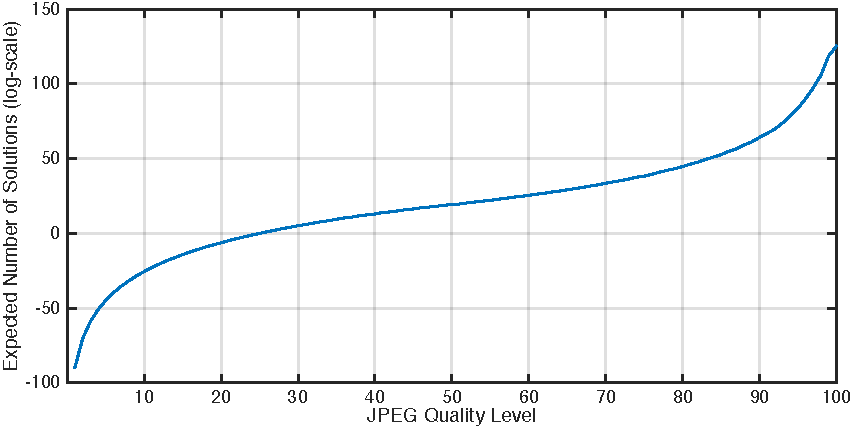
\includegraphics[width=0.8\textwidth]{figures/solcount2.pdf}\\[0em]
  \caption{Number of expected solutions}
  \label{fig:solution_count}
\end{figure}

We first tried applying CVC4, Yices, and Z3 to the problem by encoding the
problem in a format supported by the solver. We used SMT-LIB for CVC4 and Z3,
and Yices' native format for it. Unfortunately, none of these tools were able to
solve any of the problems at quality levels from $1$ to $100$ within a 1 hour
cutoff for each problem.  We also ran all three solvers without success
for over two months on problems at quality levels \(99\) and \(1\).

We have had much better success when BLT is applied to these problems.  In our
testing, BLT has been able to find solutions to all problems at quality level
\(27\) and higher.  BLT found that the problems at quality levels
\(1\) through \(18\) were \emph{unsatisfiable}. We include a chart of BLT's
runtime in Figure \ref{fig:blt-perf}. In the plot, solid points denote
problems for which BLT returns SAT, whereas $\times$ points denote problems
where BLT returns UNSAT. The large number of problems with roughly constant
runtime (mostly on the right side of the plot) have the property that the
Babai point (mentioned in section \ref{ssec:blt-optimizations}) is already a
solution and thus almost no search is needed. In the filled region between levels
19 and 26, BLT failed to terminate in the $1$ hour cutoff.

We should note that BLT is performing floating point arithmetic, and so when BLT
returns unsat there is a risk that floating point rounding error lead to BLT
detecting a branch was infeasible when it was in fact infeasible.  This may also
account for some of the performance gap, between BLT and the above solvers, but
we suspect it is unlikely that precision alone can account for the more than 6
orders of magnitude runtime difference we have observed above.

\begin{figure}[htb]
  \centering
    \includegraphics[width=0.8\textwidth]{figures/blt_benchmark.pdf}
    \caption{BLT Runtime vs. Problem Level}
    \label{fig:blt-perf}
\end{figure}

\FloatBarrier

%We have run the problem on other problems with varying constraints.
%These experiments have showna correlation between the number of expected
%solutions, and whether the solver will succeed at finding solutions.
%However, the correlation is not strict even on closely related problems.
%To illustrate this, we considered a second problem \(Q\) for which we
%added an additional row of constraints:
%
%\begin{verbatim}
%Q = { 'xx' 'xx' 'xx' 'xx' 'xx' 'xx' 'xx' 'xx'
%      'xx' '48' '65' '6c' '6c' '6f' '20' 'xx' % "Hello "
%      'xx' '57' '6f' '72' '6c' '64' '21' 'xx' % "World!"
%      'xx' 'xx' 'xx' 'xx' 'xx' 'xx' 'xx' 'xx'
%      'xx' 'xx' 'xx' 'xx' 'xx' 'xx' 'xx' 'xx'
%      'xx' '48' '65' '6c' '6c' '6f' '20' 'xx' % "Hello "
%      'xx' '57' '6f' '72' '6c' '64' '21' 'xx' % "World!"
%      'xx' 'xx' 'xx' 'xx' 'xx' 'xx' 'xx' 'xx' };
%\end{verbatim}
%
%Due to the additional rows of constraints, this problem has fewer
%solutions at a given quality level. In this case, BLT was able to find
%solutions for problems down to quality level \(68\), which was expected
%to have \(601\) solutions. In contrast, BLT was unable to solve the
%original problem \(P\) at quality level \(30\) even though that problem
%was expected to have just over \(10^{5}\) solutions. BLT was also able to
%show unsatisfiability for quality levels \(1\) through \(9\), showing
%that BLT is better able to show unsatisfiability on these problems.

%We plan to continue experiments to better understand the performance of
%BLT on different problems. Given that BLT relies on search and ILP is an
%NP-hard problem, we do not expect to be able to solve every problem, or
%even be able to accurately predict whether a particular problem can
%solved. However, research on random Boolean \(k\)-SAT problems has shown
%a clear relationships between problem satisfiability and the clause to
%variable ratio {[}3{]}. One may hope to establish similar relationships
%for bounded ILP problems.

\section{Related and Future Work}
\label{sec:final}

\textbf{Related Work}.  Our work builds upon the well-known Schnorr-Euchner
algorithm for solving the closest vector problem.  Prior to developing BLT, we
used the closest-vector solver in
\texttt{fplll}~\cite{DBLP:conf/codcry/HanrotPS11} to solve problems.  It uses
the $L^2$ norm, and thus is not a decision procedure.  However, we found that
it could often find satisfying assignments at quality levels greater than $60$
despite the lack of completeness.

\texttt{LattE} is a program for enumerating lattice points in a rational
polytope \cite{DeLoera2004}. This is asking strictly more than the question
we've discussed. \texttt{LattE} is competitive with commercial branch-and-bound
solvers, the same solvers which perform poorly on the DCT problems in section
\ref{sec:jpeg}. We attempted to evaluate \texttt{LattE} on our DCT problems,
but found that it would crash given a 16 GB memory limit.

\textbf{Future Development}.
We are still working on developing BLT, and have plans to continue
testing it on a wider variety of challenge problems.  We plan to
enable the $\linf$ distance calculation to use exact arithmetic.  We
also plan to explore ways to solve problems with one-sided bounds via
heuristics, and ways to infer unsatisfiable subsets of constraints so
that BLT can be integrated into an SMT solver.  Finally, we would like
to integrate techniques from SAT community such as
conflict-driven-clause learning into the ILP search performed by BLT.
The later should help improve its performance on hard problem instances.

More broadly, it also seems interesting to explore how the calculus and
heuristics that BLT uses can be integrated into other ILP solvers, such as those
based on cutting planes (e.g.~\cite{DBLP:journals/jar/JovanovicM13}).  Those algorithms
are able to work on more general problems as they do not require explicit upper
and lower bounds for all linear expressions.  On the other hand, BLT appears
to be more effective at making effective decisions within the search.

\textit{Acknowledgements}. The authors would like to thank Dejan Jovanovi\'{c},
Grant Passmore, and the reviewers for comments that helped improve this paper.


\bibliographystyle{plain}
\bibliography{blt-paper}

\end{document}
